\documentclass[11pt]{article}
\usepackage[utf8]{inputenc}
\usepackage[margin=1.0in]{geometry}
\usepackage{amsmath}
\usepackage{mathtools}
\usepackage{amsfonts}
\usepackage{amssymb}
\usepackage{changepage}
\usepackage{setspace}
\usepackage{verbatim}
\usepackage{xhfill}
\usepackage{sectsty}
\usepackage{enumitem}

\usepackage{color}
\newcommand{\katznote}[1]{ {\textcolor{magenta}    { ***Dan:      #1 }}}

\sectionfont{\fontsize{10}{15}\selectfont}
\renewcommand{\arraystretch}{1.5}
\setlist{noitemsep}

\begin{document}

\begin{center}
    \textbf{2018 CSE Fellowship Application - Research proposal}
\hfill
\textbf{Joshua Vita}
\end{center}
\noindent\hrulefill

\bigskip

With the rise of modern computers, many fields in science and engineering have grown to include sub-fields designed to incorporate new computational methods. Computational materials science is one such sub-field, focused on exploring materials systems by using computers to simulate atomic interactions. In general, there are two approaches to modeling atomic interactions: a ``first-principles'' quantum mechanical approach based on electron-electron interactions, and empirical potentials that coarse-grain out the electronic degrees of freedom. While first-principles techniques can accurately predict material properties, they are significantly restricted due to the computational complexity associated with solving for electronic interactions: typically $\sim10^2-10^3$ atoms for at most $10^{-11}\text{s}$. Reaching larger length- and time-scales necessary for the design of next generation materials requires empirical potentials that achieve nearly as accurate predictions of quantum mechanical methods at a fraction of the computational effort.

%%% DRT: this is a strange sentence; e.g., one can do MD with first-principles calculation of forces
% On the other hand, molecular dynamics relies solely on Newtonian mechanics; by calculating the energies and forces on an atom, it is relatively simple to perform time integration on Newton's equations of motion in order to simulation atomic movement.

In computational materials science, empirical potentials are a fundamental element of multiscale modeling. An empirical potential is a function that calculates energies and forces on atoms depending on various properties of the atomic environment, such as interatomic spacing or chemistries of atoms. These functions sometimes can have explicit algebraic formulations, though not all of them do. Through the use of empirical potentials, molecular dynamics simulations have been able to access system sizes on the order of $10^6-10^9$ atoms and timescales of nano- to micro-seconds (or even longer), impacting a wide array of fields, from materials science and physics to chemistry and even biology. My current work aims to build a massively parallel optimization engine that leverages not only the petascale computing powers available to us, but also the rapidly-growing materials databases that are being built by the community. My goal is to develop the ability to create accurate, robust potentials without sacrificing significant amounts of human effort.

% \bigskip

Not only would this work be significant because of how it would help push potential fitting onto supercomputing platforms, but also because of how much it could lower the barrier to entry for exploration into new materials systems. Standard methods of developing empirical potentials (even taking into account popular potential fitting software \cite{potfit}) are sometimes described as a type of ``black magic" since they require a large amount of intuition and fine-tuning by experts in the field. The biggest challenge in this technique is selecting the optimal set of atomic configurations to fit against in order to accurately model the physical and chemical processes of interest (we will refer to the method of choosing a set of configurations as `database optimization').

Due to the necessary cycle of fitting, testing, and retesting a potential, the production of a `good' interatomic potential takes months or even years of work. Because of this, it can be difficult for researchers to begin working with a system that hasn't already been modeled by an existing empirical potential. Since materials research is largely driven by a desire to discover new materials, this barrier associated with developing new empirical potentials has a strong impact on scientific progress in the field. The possibility for rapid development of potentials, as is the goal in my work, would encourage investigation into newer and more complex systems, which would in turn influence many fields in science and engineering.

% \bigskip

In previous work, our group developed a new approach to database optimization that utilizes Bayesian inference \cite{baye} and Markov Chain Monte Carlo methods to iteratively select the optimal subset of a materials database \cite{dbopt}. This method, outlined in Figure \ref{fig:workflow}, effectively reduces the need for human intervention and guesswork associated with the fitting process, potentially condensing years of costly research time into a simple matter of computer walltime. As a proof-of-concept, we used this new algorithm to augment an existing titanium potential to include titanium-oxygen interactions, creating a useful binary potential \cite{tio}. While this previous work demonstrated the value of the algorithm, my work aims to build the tools needed to scale the algorithm up into a more usable state.

\begin{figure}
  \centering
  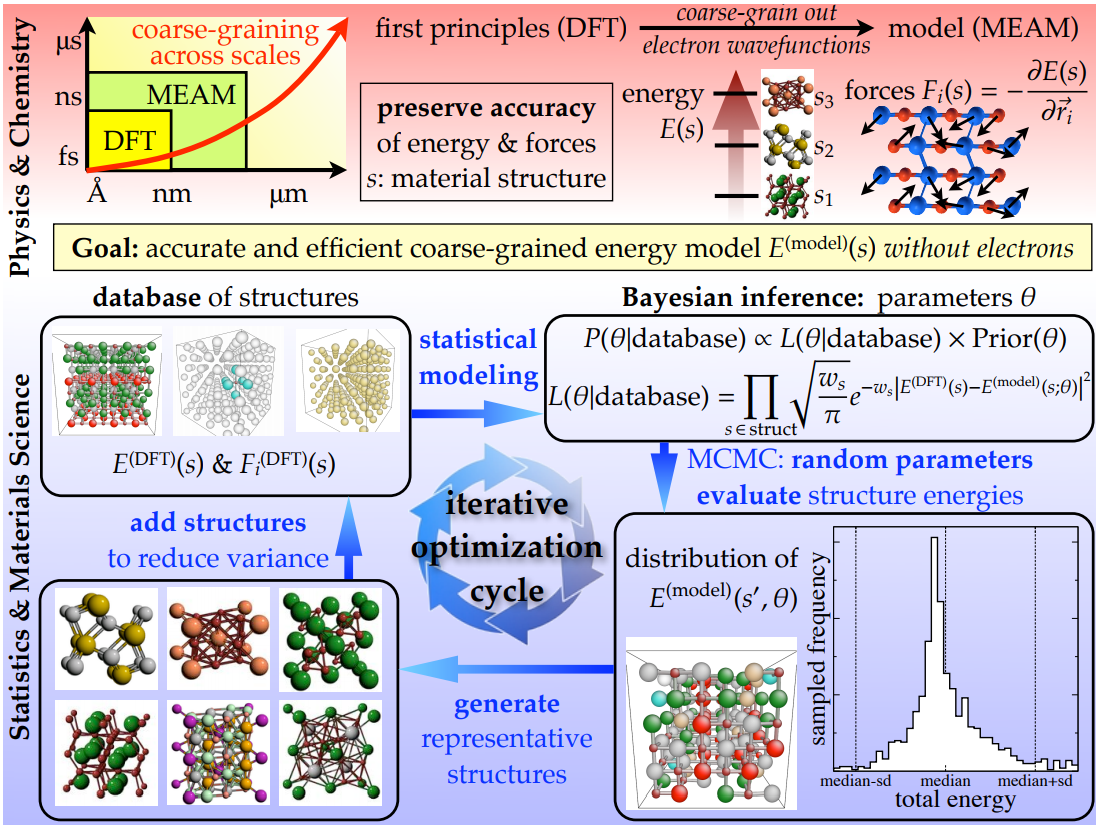
\includegraphics[width=0.65\linewidth]{workflow.png}
  \caption{\textit{A general overview of the workflow demonstrated by previous work in our group \cite{dbopt}. Integral to the scalability of this process, and the purpose of the currently proposed work, is to design a massively parallel evaluation engine for rapid evaluation of energies and forces of all structures in the database.}}
  \label{fig:workflow}
\end{figure}

At the center of this algorithm, or related algorithms that I could develop in the future, there needs to be a massively parallel evaluation engine that takes a list of structures (atomic positions and chemistries), and a large vector of parameters for the empirical potential, and evaluates the energies and forces of each structure for each parameter set. As more parameters and structures are included into the database, the need for a massively parallel approach becomes readily apparent. For example, if we consider

\begin{itemize}
    \item $\mathbf{10^6}$ potential parameters, which is on the order needed for Bayesian sampling, applied to
    \item $\mathbf{10^3}$ atomic configurations
\end{itemize}

\noindent Then while each individual calculation may require mere milliseconds to complete, we have approximately $10^9$ computations requiring multiple terabytes of data being used simultaneously. While these calculations are, fortunately, embarrassingly parallelizable and can be executed with a master-worker approach, advanced algorithms are required to properly handle the parallel workflow and the large amounts of simultaneous data. Nevertheless, if we are able to achieve these larger scales, the structural and energy landscapes of an empirical potential could be fully analyzed in order to produce accurate, predictive, and transferable empirical potentials. This would lower the barrier to entry for researchers interested in new materials systems, encouraging the exploration of novel materials and strengthening the field of computational materials science as a whole.

This task transforms a purely materials science problem (potential fitting) into an interdisciplinary challenge requiring expertise and collaboration in the fields of high performance computing and software development for massively parallel applications. The goal of achieving petascale parallelization is on its own something that has been rarely achieved in computational materials science in general and remains largely untouched in terms of potential fitting in particular. Success would be a meaningful step in the field of materials modeling towards proper utilization of cutting-edge supercomputing capabilities.

The purpose of my current work is to design and implement such a massively parallel evaluation, to be used as the framework through which to deploy our new algorithm. A key element in my work was the choice to use a spline-based modified embedded-atom method (MEAM) potential form, which allows for some unique optimization techniques. In my work so far, I have created a highly optimized version of the worker in the master-worker paradigm. I have also come up with a novel way of storing atomic structural information for use with spline MEAM potentials that reduces the number of calculations that have to be performed by tens or hundreds of times. My next step will be to begin the parallelization process, working towards deployment on Blue Waters.

Beyond its impact in the scientific community, I also see this work as a critical step in my professional development. Ever since the early years of my college career, I've focused on advancing my skills in software development and mathematics, with the broad goal of someday being able to apply them towards real-world scientific problems. While my interests have always been intimately tied to the questions being asked by materials scientists, I also love the experience of getting to build new, innovative, and powerful pieces of software in order to answer those questions. My work here at the University of Illinois is the perfect opportunity for me to use my skills to make a profound contribution to the field.

In addition to being a way of providing a useful tool to my community, this work has also introduced me to the burgeoning field of research software engineering; a subset of software development that is specifically focused on software applications in research. This society is populated by like-minded individuals who are driven to solve problems from physics, chemistry, and engineering through the use of computer programming. My goal over the next few years is to prepare myself to be able to contribute to large-scale collaborative efforts in scientific software development. I see my current work as an opportunity not only to refine my technical skills (in terms of coding and good software development practices), but also as a chance to gain more experience in collaborative development and software deployment on high performance computers.

Given the inherently interdisciplinary nature of my work and its potential for wide-reaching impacts, I think that it will serve as an excellent example of the type of work being done by the CSE community here on campus. Not only does it provide a clear link between materials science and petascale computing, but it also could fundamentally change how researchers broach the task of exploring a whole class of materials systems. On a more personal level, working on this project is the perfect conduit through which to further my goals of being able to contribute to society as a research software engineer. Thank you for taking the time to consider my proposal; I look forward to continuing to contribute to the CSE community and to seeing all of the impressive work being done by next year's CSE Fellows.

\bibliography{bibliography}
\bibliographystyle{plain}

\end{document}
